\begin{frame}{Definiciones}
	\dificultyLevel{2}
	\begin{itemize}
		\item Sean $X$ los features y $ent(x)$ el conjunto de entidades.
		\item Luego $M$ es el modelo y $\phi$ un \textit{feature attribution score}
	\end{itemize}
	\begin{figure}
		\centering
		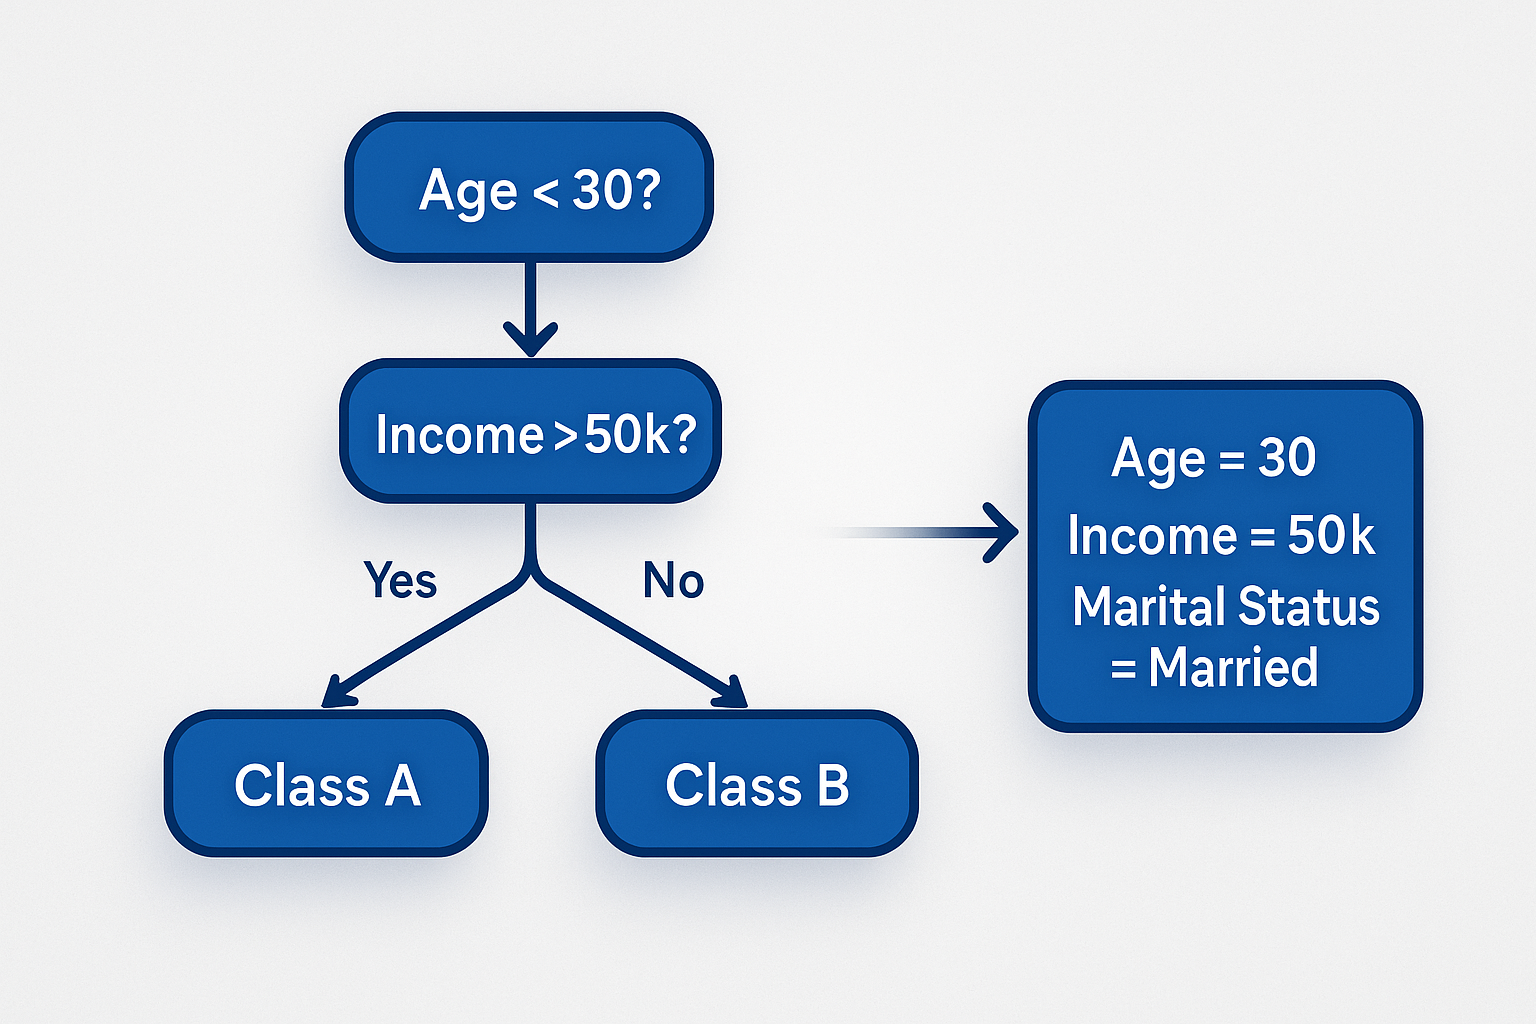
\includegraphics[width=0.7\linewidth]{pic/img/XAI/modelAndEntityExample.png}
	\end{figure}
\end{frame}


\begin{comment}
	\begin{frame}{Definiciones}
		\dificultyLevel{2}
		\begin{mydefinition}[Entidades]
			Sea $X$ el conjunto de features, definimos a $ent(X)$ cómo el conjunto de todas las entidades, con un espacio de probabilidad definido por una distribución $Pr$.
		\end{mydefinition}
	\end{frame}
	
	\begin{frame}{Definiciones}
		\begin{mydefinition}[Modelo]
			Un modelo $M$ es una función  $\phi : ent(X) \to \set{0,1}$, que dada una entidad $e$ devuelve 0 o 1, siendo esta su clasificación.
		\end{mydefinition}
		\begin{mydefinition}[Feature attribution score]
			Un \textit{feature attribution score} es una función $\phi : X \to \mathbb{R}$, esta indica la \textit{relevancia} de cada feature con respecto a una predicción $M(e)$.
		\end{mydefinition}
	\end{frame}
\end{comment}

\begin{frame}{Shapley Values}
    \dificultyLevel{2}
    \textbf{SHAP} se basa en los \textit{Shapley Values} de teoría de juegos cooperativos. Podemos interpretar a este valor $\phi_i(\charactheristicFunction)$ como el aporte del jugador $i$ al juego definido por la función $\charactheristicFunction$.
\end{frame}

\begin{frame}{Asado Familiar : Subconjunto original}
		\begin{figure}
		\centering
		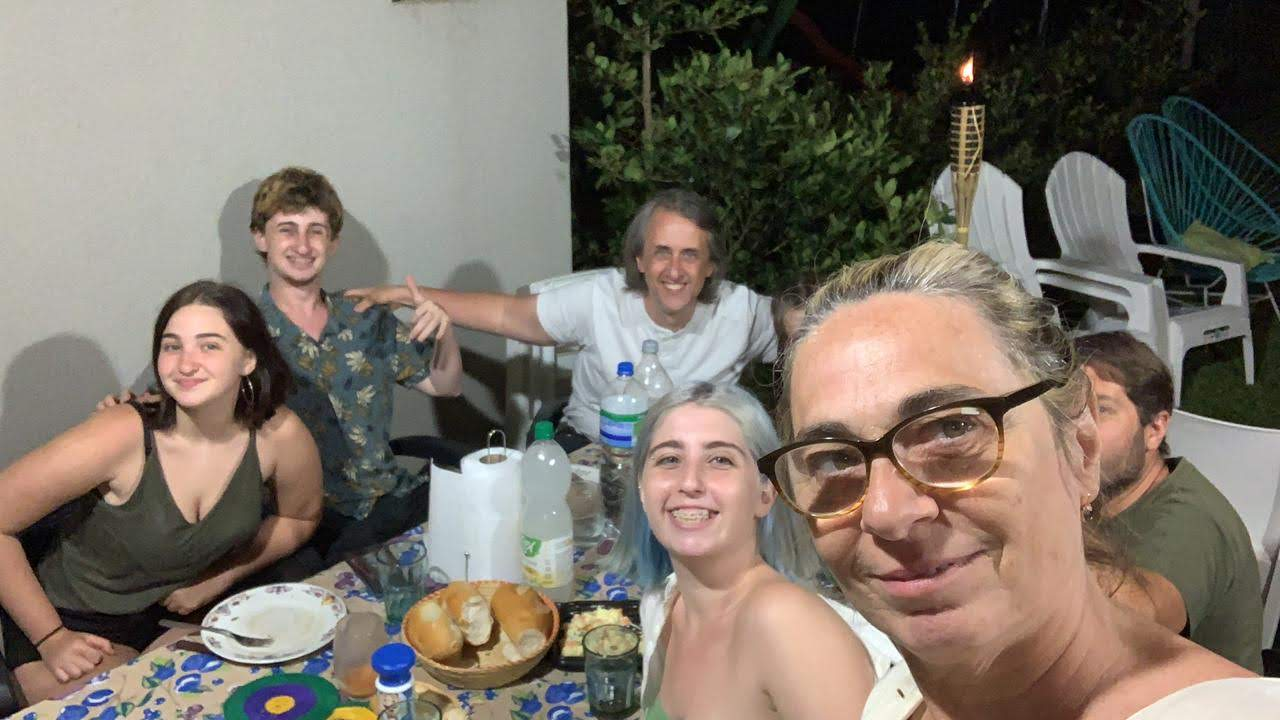
\includegraphics[width=0.9\linewidth]{pic/img/XAI/subconjuntoTotal.jpg}
	\end{figure}
\end{frame}

\begin{frame}{Asado Familiar : Subconjunto óptimo}
	\begin{figure}
		\centering
		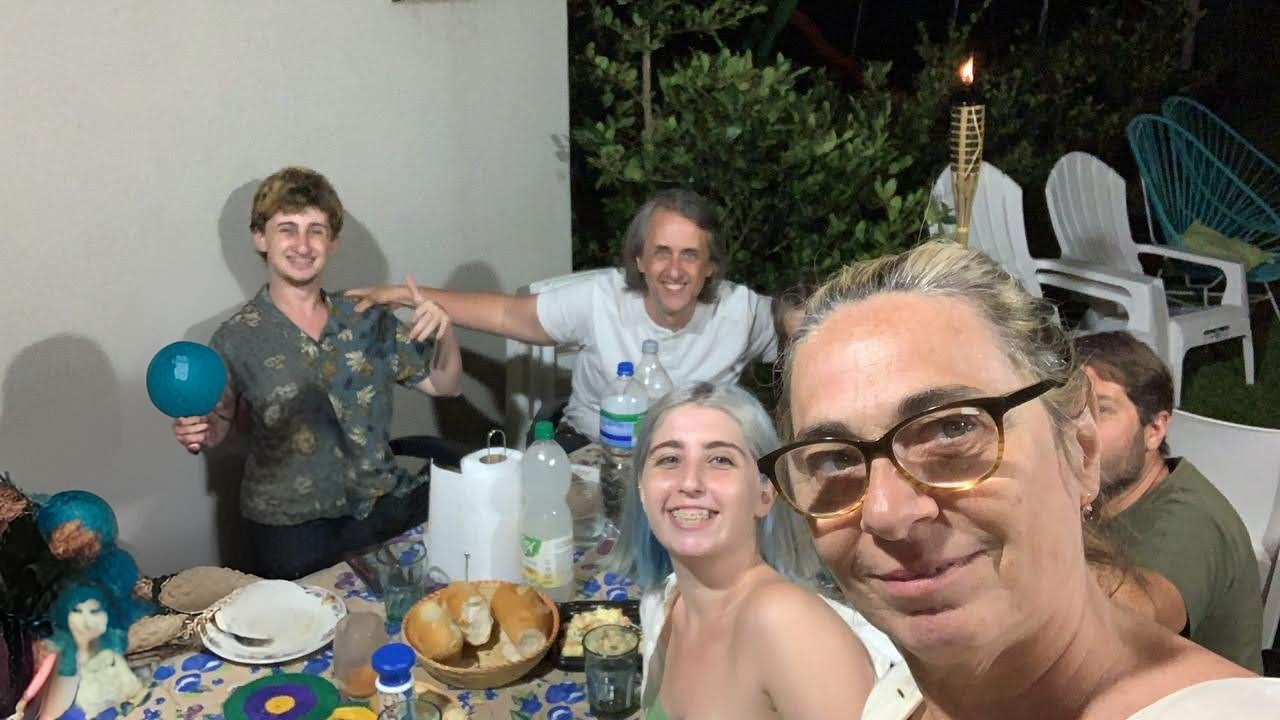
\includegraphics[width=0.9\linewidth]{pic/img/XAI/subconjuntoOptimo.png}
	\end{figure}
\end{frame}

\begin{comment}
	Definición Shapley Values: Ejemplo
	El "Juego": Medir el nivel de éxito y disfrute de un asado familiar, en una escala del 1 (intoxicación masiva) al 10 (gloria culinaria). La "predicción base" o el resultado promedio de cualquier juntada es un 6.
	Los "Jugadores" (Features):
	El que pone la casa y la parrilla.
	El que trae una ensalada de rúcula y parmesano espectacular.
	La que compra un vino de calidad cuestionable.
	Tu hermana (jugador i), que no trajo nada, usó tu silla preferida y se quejó del punto de la carne.
	
\end{comment}

\begin{frame}{Propiedades Shapley Values}
	Las propiedades de los \textit{Shapley Values} son:
	\begin{itemize}
		\item \textbf{Eficiencia:} Toda la ganancia es distribuida 
		%La sumatoria de los shapley values para cada feature es igual a la predicción promedio del modelo. 
		\item \textbf{Simetría:} Jugadores equivalentes reciben el mismo valor.  
		%Si para todas las coaliciones a las que se suman estos jugadores, su valor es el mismo -> tienen el mismo shapley value
		\item \textbf{Linealidad:} El valor de Shapley es lineal respecto a la función característica. 
		% Podes sumar y multiplicar las funciones características, y los shapley values se verán linealmente afectados.  -> \phi_i(a \v + \v2) =  a \phi_i(\v) + \phi_i(\v2)
		\item \textbf{Jugador Nulo:} Si no aporta, su valor es 0.
	\end{itemize}
\end{frame}

\begin{frame}{Fórmula Shapley}
	\dificultyLevel{3}
	\textbf{Fórmula general:}
	
	% Parte visual progresiva de la fórmula
	\only<1,2>{%
		\begin{mydefinition}[Shapley Value]
			\[
			\phi_i(\charactheristicFunction) = \text{Shapley Value del jugador $i$ para la función $\charactheristicFunction$}
			\]
		\end{mydefinition}
	}
	\only<3>{%
		\begin{mydefinition}[Shapley Value]
			\[
			\phi_i(\charactheristicFunction) = \alert<3>{\charactheristicFunction(\pi_{<i}\cup\{i\}) - \charactheristicFunction(\pi_{<i})}
			\]
		\end{mydefinition}
	}
	\only<4>{%
		\begin{mydefinition}[Shapley Value]
			\[
			\phi_i(\charactheristicFunction) = \alert<4>{\sum_{\pi \in perm(X)}}\; \charactheristicFunction(\pi_{<i}\cup\{i\}) - \charactheristicFunction(\pi_{<i})
			\]
		\end{mydefinition}
	}
	\only<5>{%
		\begin{mydefinition}[Shapley Value]
			\[
			\phi_i(\charactheristicFunction) = \alert<5>{\frac{1}{|X|!}}\; \sum_{\pi \in perm(X)} \bigl(\charactheristicFunction(\pi_{<i}\cup\{i\}) - \charactheristicFunction(\pi_{<i})\bigr)
			\]
		\end{mydefinition}
	}
	
	\only<2>{
		\begin{mydefinition}
			La función característica se define como:
			\[
			\charactheristicFunction : \mathcal{P}(X) \to \mathbb{R}
			\]
			Asigna un real a cada posible \textit{coalición} de jugadores, es decir, a cada subconjunto de \( X \).
		\end{mydefinition}
	}
	
	% Lista explicativa
	\begin{itemize}
		\item<3-> \alert<3>{Se calcula cuánto colabora $i$ a $\pi$: $\charactheristicFunction(\pi_{<i}\cup\{i\})-\charactheristicFunction(\pi_{<i})$.}
		\item<4-> \alert<4>{Se suman todas las permutaciones de $X$, para ver cuánto colabora $i$ a cada una.}
		\item<5-> \alert<5>{Se divide todo por $|X|!$, porque se está promediando sobre todas las permutaciones posibles.}
	\end{itemize}
\end{frame}


\begin{comment}

	\begin{frame}{Fórmula función característica en ML}
		\dificultyLevel{3}
		% Parte visual progresiva de la fórmula
		\only<1>{%
			\begin{mydefinition}[Función característica]
				\scriptsize
				\[
				v_{M,e,\Pr}(S) = \text{Predicción promedio de $M$ cuando los features $S$ toman los valores de $e$}
				\]
			\end{mydefinition}
		}
		\only<2>{%
			\begin{mydefinition}[Función característica]
				\[
				v_{M,e,\Pr}(S) = \alert<2>{\sum_{e' \in \consistsWith(e,S)}} \cdots
				\]
			\end{mydefinition}
		}
		\only<3>{%
			\begin{mydefinition}[Función característica]
				\[
				v_{M,e,\Pr}(S) = \sum_{e' \in \consistsWith(e,S)} \alert<3>{\Pr[e'|\consistsWith(e,S)]} \cdot \cdots
				\]
			\end{mydefinition}
		}
		\only<4,5>{%
			\begin{mydefinition}[Función característica]
				\[
				v_{M,e,\Pr}(S) = \sum_{e' \in \consistsWith(e,S)} \Pr[e'|\consistsWith(e,S)] \cdot \alert<4>{M(e')}
				\]
			\end{mydefinition}
		}
		
		% Lista explicativa
		\begin{itemize}
			\item<2-> \alert<2>{Se consideran las instancias $e'$ que coinciden con la entidad $e$ en los atributos de $S$: $\consistsWith(e,S)$.}
			\item<3-> \alert<3>{Se pondera cada $e'$ según su probabilidad condicional dado que coincide con $e$ en $S$: $\Pr[e'|\consistsWith(e,S)]$.}
			\item<4-> \alert<4>{Se evalúa el modelo $M$ sobre cada $e'$.}
			\item<5-> \alert<5>{En resumen: $v(S)$ es la predicción promedio del modelo dejando fijos los features de $S$.}
		\end{itemize}
	\end{frame}
\end{comment}



\begin{frame}{SHAP en Aprendizaje Automático}
\dificultyLevel{2}
	\begin{itemize}
	    \item Features $X$ son los jugadores, y $\charactheristicFunction_{M,e,Pr}(S)$ es la predicción promedio.
	    %\item Utilizamos la fórmula $c_m$ para agrupar permutaciones con el mismo subconjunto. 
	    \item Así la fórmula de SHAP nos queda: \pause
	    %\item Por último utilizando la notación $c_m = \frac{m! (|X|-m-1!)}{|X|!}$, podemos encontrar la fórmula de Shap. \pause 
	    \begin{mydefinition}[SHAP]
	    Teniendo un modelo $M$, una entidad $e$, un feature $x_i$ y una función de probabilidad $Pr$ definimos $\Shap$ como:
	    \[ \Shap_{M,e,\Pr}(x_i) = \sum_{S \subseteq X \setminus \{x_i\}} c_{|S|} (\charactheristicFunction(S \cup \{x_i\}) - \charactheristicFunction(S)) \]    
	    \end{mydefinition}
	    %Mencionar las críticas a SHAP cómo:
	        %Nótese que los axiomas que estos valores satisfacen no tienen un significado claro en el contexto de la inteligencia artificial, ya que dependen de la definición de v[10]. Además, para algunas nociones simples y robustas de atribución de características basadas en explicaciones abductivas [22], los valores de Shapley no logran asignar un puntaje de 0 a features irrelevantes [11].
	    
	\end{itemize}
\end{frame}

% Slide 1: Motivación y definición general
\begin{frame}{Asymmetric Shapley Values (ASV)}
\dificultyLevel{2}

\begin{itemize}[<+- | alert@+>]
	\item La definición clásica de Shapley values asigna el \textbf{mismo peso a todas las permutaciones}.
	\item En ASV se busca \textbf{asignarle más peso a ciertas permutaciones}.  
	\item Para capturar esta idea \textbf{relajamos la propiedad de la simetría}, definiendo una función de peso $w$ sobre las permutaciones
	%\[	w : \perm(\players) \to \R 	\quad\text{con}\quad 	\sum_{\pi} w(\pi)=1\,, 	\]
\end{itemize}
%Sin embargo, cuando hay relaciones causales entre features, algunos órdenes no son coherentes (p.ej. evaluar “educación” antes que “edad”).  


\end{frame}

\begin{frame}{Definición formal de ASV}
\dificultyLevel{3}

\begin{mydefinition}[Asymmetric Shapley Values]
Dada una función característica
\(\;\charactheristicFunction : \mathcal{P}(\players)\to\R\)\; y un peso \(w\) sobre permutaciones, los ASV son
\[
\phi^{assym}_i(v)
\;=\;
\sum_{\pi \in \perm(\players)} 
   \alert{w(\pi)}\bigl(\charactheristicFunction(\pi_{<i}\cup\{i\})-\charactheristicFunction(\pi_{<i})\bigr).
\]
\end{mydefinition}

\end{frame}

\begin{frame}{Ejemplo : Naive Bayes como DAG causal}
\dificultyLevel{2}
    \begin{figure}[ht]
    \centering
    \scalebox{0.8}{
        \begin{tikzpicture}[
            every node/.style={circle, minimum size=1.2cm, font=\small, text=white},
            class/.style={draw, fill=red!70},
            feature/.style={draw, fill=blue!60},
            node distance=1.8cm and 1.8cm,
            ->, thick
        ]
    
            % Central class node
            \node[class] (Disease) {Enfermo};
    
            % Features aligned horizontally below
            \node[feature, below left=of Disease, xshift=-3.6cm] (Fever) {Fiebre};
            \node[feature, right=of Fever] (Cough) {Tos};
            \node[feature, right=of Cough] (Fatigue) {Fatiga};
            \node[feature, right=of Fatigue] (Test) {Dolor};
            \node[feature, right=of Test] (Age) {Edad};
    
            % Edges
            \draw (Disease) -- (Fever);
            \draw (Disease) -- (Cough);
            \draw (Disease) -- (Fatigue);
            \draw (Disease) -- (Test);
            \draw (Disease) -- (Age);
    
        \end{tikzpicture}
    }
	\end{figure}
    
   % \pause     
    %\begin{itemize}     	\item En el caso que nuestro DAG $G$ fuera esta red de ejemplo, las únicas permutaciones válidas serían las cuáles contengan al nodo \textbf{Enfermo} primero.     \end{itemize}
\end{frame}


\begin{frame}{Función de peso desde un DAG causal}
	\dificultyLevel{2}
	
	Dado un DAG causal \(G=(X,E)\). El conjunto de \textbf{órdenes topológicos} son las permutaciones que respetan al grafo causal. % \(\topo(G)\subseteq\perm(X)\).
	\begin{figure}
		\centering
		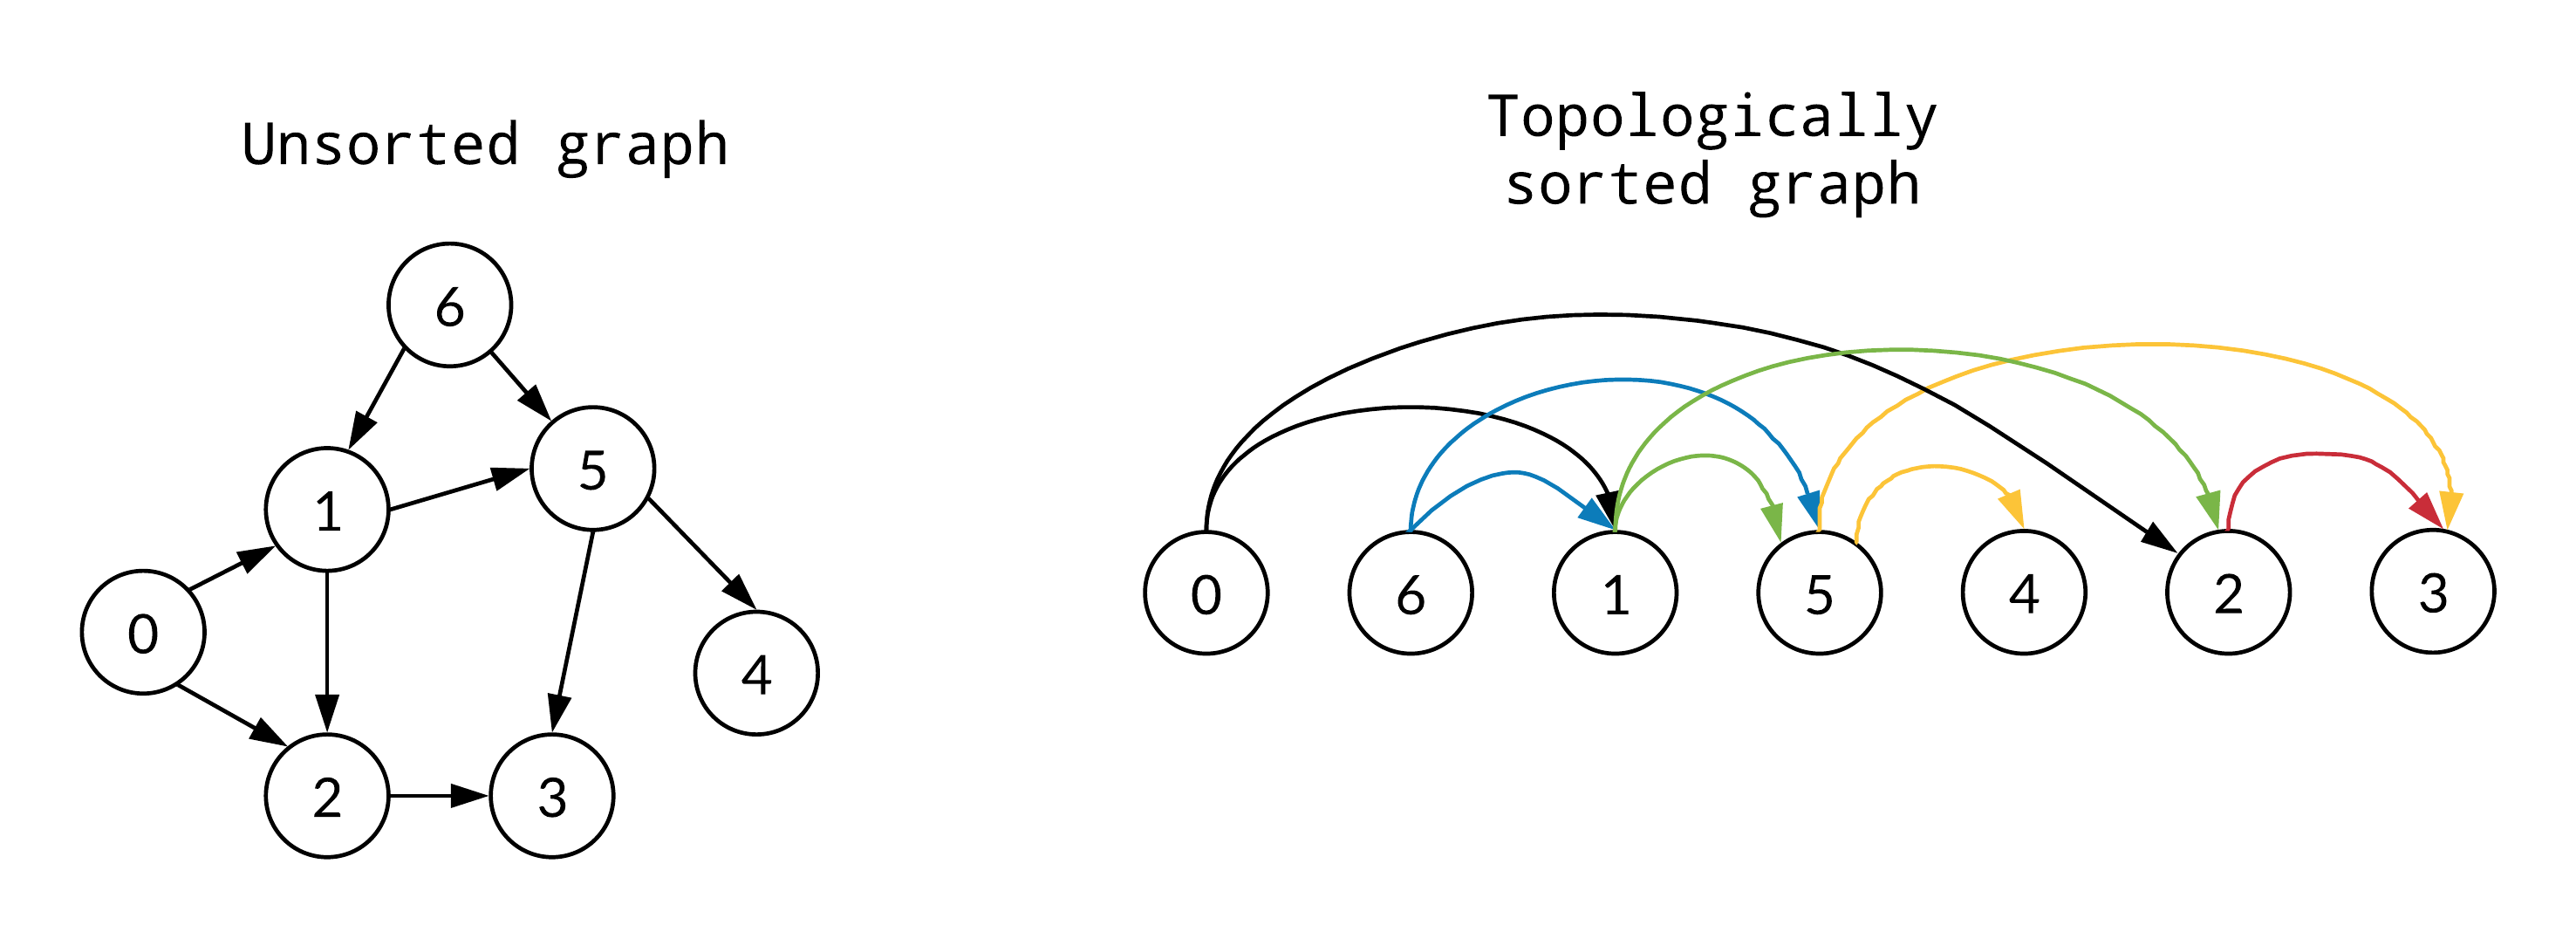
\includegraphics[width=0.9\linewidth]{pic/img/SHAP/topologicalSortExample.png}
	\end{figure}
\end{frame} 

\begin{comment}
		\only<2>{
		\begin{mydefinition}[Orden topológico]
			Dado un grafo dirigido acíclico (DAG) \(G = (V, E)\), un orden topológico es una permutación \(\pi\) de los nodos \(V\) tal que para toda arista \((u, v) \in E\), se cumple que \(\pi(u) < \pi(v)\).
			
			Esto garantiza que todo nodo aparece después de sus predecesores en el grafo.
		\end{mydefinition}
	}
\end{comment}

\begin{frame}{Función de peso desde un DAG causal}
	\dificultyLevel{3}
	
	Así es como \textbf{cada orden recibe el mismo peso}, y cada permutación que \textbf{no es un orden tópologico no debe ser contabilizada}. De esta forma $w$ nos queda:
	\[
	w(\pi)=
	\begin{cases}
		\displaystyle \tfrac1{|\topo(G)|},&\pi\in\topo(G),\\
		0,&\text{en otro caso.}
	\end{cases}
	\]
	
\end{frame}


\begin{frame}{ASV en aprendizaje automático}
	\dificultyLevel{3}
	
	\begin{mydefinition}[ASV con DAG Causal]
		%Teniendo un modelo \(M\), una entidad \(e\), un feature \(x_i\), una función de probabilidad \(\Pr\), y un DAG causal \(G\) sobre los features, definimos \(\assym\) como: \pause
		\[
		\assym_{M,e,\Pr}(x_i) = \alert{\frac{1}{|\topo(G)|}} \sum_{\alert{\pi \in \topo(G)}} \left( \charactheristicFunction(\pi_{<i} \cup \{x_i\}) - \charactheristicFunction(\pi_{<i}) \right)
		\]
	\end{mydefinition}
	\pause
	\begin{itemize}[<+- | alert@+>]
		\item Es la misma fórmula que SHAP, solo que tomamos las permutaciones que sean órdenes topológicos
		\item Este enfoque prioriza las permutaciones causalmente válidas y \textit{asigna más importancia} a las causas que a las consecuencias.
	\end{itemize}
	
\end{frame}

%TODO: Meter meme de basta de fórmulas o algo por el estilo

\begin{comment}
	\begin{frame}{Complejidad Computacional de SHAP y ASV}
		\dificultyLevel{3}
		En ~\cite{van2022tractability} Guy Van et al. demostraron que:
		\begin{itemize}[<+- | alert@+>]
			\item El cálculo general de SHAP es $\sharpPhard$.
			\item Con la distribución \textit{empírica}, SHAP es $\sharpPhard$ incluso para árboles.
			\item Con la distribución Naive Bayes con modelo trivial $f(x)=x_1$, también es $\sharpPhard$.
			\item SHAP es tratable para una familia de modelos bajo distribución \textit{producto} sii el promedio es tratable
		\end{itemize}
		
	\end{frame}
\end{comment}

\begin{comment}
	\item Formalmente, si \(X = \{x_1, \ldots, x_n\}\), con raíz \(x_1\), entonces:
	\[
	\Pr[e] = \Pr[x_1 = e(x_1)] \cdot \prod_{j=2}^{n} \Pr[x_j = e(x_j) \mid x_1 = e(x_1)]
	\]
\end{comment}

\begin{comment}
	\begin{frame}{Ejemplo: Distribución Naive Bayes}
		\dificultyLevel{2}
		
		\begin{itemize}
			\item Una red Naive Bayes define una \textbf{distribución de probabilidad sobre entidades } \(e\), basada en un nodo raíz que condiciona a todos los demás. \pause
			
			\item En nuestro contexto, usamos esta \textbf{distribución como la \(\Pr\) y $DAG$ causal} de nuestras entidades. Podría ocurrir que el grafo causal sea distinto a esta red. 
		\end{itemize}
		
		\begin{figure}[ht]
			\centering
			\scalebox{0.6}{
				\begin{tikzpicture}[
					every node/.style={circle, minimum size=1.2cm, font=\small, text=white},
					class/.style={draw, fill=red!70},
					feature/.style={draw, fill=blue!60},
					node distance=1.8cm and 1.8cm,
					->, thick
					]
					% Central class node
					\node[class] (Disease) {Enfermo};
					
					% Features aligned horizontally below
					\node[feature, below left=of Disease, xshift=-3.6cm] (Fever) {Fiebre};
					\node[feature, right=of Fever] (Cough) {Tos};
					\node[feature, right=of Cough] (Fatigue) {Fatiga};
					\node[feature, right=of Fatigue] (Test) {Dolor};
					\node[feature, right=of Test] (Age) {Edad};
					
					% Edges
					\draw (Disease) -- (Fever);
					\draw (Disease) -- (Cough);
					\draw (Disease) -- (Fatigue);
					\draw (Disease) -- (Test);
					\draw (Disease) -- (Age);
				\end{tikzpicture}
			}
		\end{figure}
	\end{frame}
\end{comment}


\begin{frame}{Complejidad de ASV}
	\dificultyLevel{2}
	Nuestro objetivo es estudiar la \textbf{tratabilidad} de ASV para los casos que SHAP no es tratable.Luego teniendo en cuenta que: \pause 
	
	\begin{itemize}[<+- | alert@+>]
		\item El conjunto sobre el cual se itera en ASV es más reducido que el de SHAP
		\item La distribución Naive Bayes se asemeja a una producto.
	\end{itemize}
	
	\pause
	llegamos a nuestro primer resultado: 
	\begin{mytheorem}[Tratabilidad de ASV]
		\small
		ASV puede calcularse en tiempo polinomial bajo una distribución Naive Bayes para una familia de modelos $\mathcal{F}$ si y solo si SHAP puede calcularse para $\mathcal{F}$ bajo distribución producto.
	\end{mytheorem}
\end{frame}

\begin{frame}{Objetivo de la tesis}
	\dificultyLevel{2}
	\begin{itemize}[<+- | alert@+>]
		\item A raíz del teorema anterior surge el objetivo inicial de la tesis, el cuál era realizar \emph{el cálculo exacto de ASV en tiempo polinomial para una red bayesiana.} 
		\item Como vamos a necesitar evaluar a $\charactheristicFunction$, necesitamos un modelo el cual pueda calcular el promedio en tiempo polinomial. Por eso nos vamos a centrar en \textbf{árboles de decisión.}
		\item El cálculo del promedio va a depender de su distribución $Pr$, que en este caso es una \textbf{Red Bayesiana}. 
		%\item Por lo que es necesario entender estas distribuciones para poder realizar este cálculo. 
	\end{itemize}
	
\end{frame}